\documentclass[11pt,a4paper]{article}

\usepackage[T1]{fontenc}
\usepackage[utf8]{inputenc}
\usepackage[a4paper,margin=1in]{geometry}
\usepackage{lmodern}
\usepackage{microtype}
\usepackage{amsmath,amssymb,amsthm,mathtools}
\usepackage{booktabs}
\usepackage{graphicx}
\usepackage{enumitem}
\newtheorem{theorem}{Theorem}
\newtheorem{lemma}{Lemma}
\newtheorem{corollary}{Corollary}
\newtheorem{proposition}{Proposition}
\newtheorem{remark}{Remark}
\newtheorem{definition}{Definition}

\DeclareMathOperator{\Pois}{Pois}
\DeclareMathOperator{\LambertW}{W}

\newcommand{\RR}{\mathbb{R}}
\newcommand{\cF}{\mathcal{F}}
\newcommand{\barr}{\bar r}
\newcommand{\barR}{\bar R}
\newcommand{\barp}{\bar p}
\newcommand{\alg}{\mathsf{Alg}}
\newcommand{\opt}{\mathsf{Opt}}
\newcommand{\e}{\mathrm e}

\title{Robust last-success stopping with predicted odds\\
\large Detailed notes: independent discrete trials and the continuous Poisson limit}
\author{}
\date{}

\begin{document}
\maketitle

\begin{abstract}
We study the problem of stopping on the last success.  In the independent
finite model, Bruss' odds theorem says that the optimal policy is obtained by
summing the true odds from the end until reaching one.  We then assume that only
predicted odds are available and that the predictions are multiplicatively
\(\rho\)-accurate.  We prove finite-\(n\) robustness bounds for threshold rules
that sum predicted odds up to a target \(\theta\), optimize this target, and
compare it with the naive target \(\theta=1\).  We also clarify that this optimized threshold is not a global minimax rule over randomized strategies, give an exact two-period counterexample, and record the corresponding semi-infinite linear programming formulation.  We then derive the analogous and
cleaner result for the continuous Poisson model, where the state is summarized
by the remaining intensity mass.  Finally, we add a Bayesian model in which local
multiplicative errors are drawn independently from a known law; in that case the
optimal rule is again exactly Bruss' rule, applied to induced effective odds.
\end{abstract}

\section{The basic last-success problem}

Let \(I_1,\dots,I_n\) be Bernoulli indicators.  A success occurs at time \(i\)
when \(I_i=1\).  The goal is to choose a stopping time \(\tau\) and maximize
\[
  \mathbb P\bigl(I_\tau=1,\ I_{\tau+1}=\cdots=I_n=0\bigr),
\]
that is, the probability of stopping exactly on the last success.

In the independent model, write
\[
  p_i=\mathbb P(I_i=1),\qquad q_i=1-p_i,\qquad
  r_i=\frac{p_i}{q_i}.
\]
The number \(r_i\) is the \emph{odd} of a success at time \(i\).  For
\(k\in\{1,\dots,n\}\), define the true tail odds and the true tail failure
product by
\[
  R_k=\sum_{j=k}^n r_j,\qquad
  Q_k=\prod_{j=k}^n q_j=\prod_{j=k}^n \frac1{1+r_j}.
\]
We also use the convention \(R_{n+1}=0\) and \(Q_{n+1}=1\).

\begin{lemma}[Value of a deterministic threshold]
\label{lem:threshold-value}
Assume that \(I_1,\dots,I_n\) are independent.  If the policy ignores all
successes before \(k\) and then stops at the first success in
\(\{k,k+1,\dots,n\}\), its success probability is
\[
  W(k)=Q_kR_k.
\]
\end{lemma}

\begin{proof}
The policy wins if and only if there is exactly one success in the tail
\(\{k,\dots,n\}\).  By independence,
\begin{align*}
  \mathbb P(\text{exactly one success in }\{k,\dots,n\})
  &=\sum_{i=k}^n p_i\prod_{\substack{j=k\\j\ne i}}^n q_j \\
  &=\left(\prod_{j=k}^n q_j\right)
    \sum_{i=k}^n \frac{p_i}{q_i} \\
  &=Q_kR_k.
\end{align*}
This proves the claim.
\end{proof}

\begin{theorem}[Bruss' odds theorem, threshold form]
\label{thm:bruss}
Assume that the indicators are independent.  In the non-degenerate case
\(R_1>1\), an optimal rule is the following: let
\[
  s=\sup\left\{k\in\{1,
  \dots,n\}:R_k=\sum_{j=k}^n r_j\ge1\right\}.
\]
Equivalently,
\[
  R_s\ge1>R_{s+1}.
\]
Then it is optimal to ignore all successes before \(s\), and to stop at the
first success from \(s\) onward.  The optimal value is
\[
  V^\star=Q_sR_s.
\]
If \(R_1<1\), then the optimal rule starts at \(1\), i.e. it stops at the first
success.
\end{theorem}

The theorem is due to Bruss (2000).  The main message is that one
sums \emph{odds}, not success probabilities.  When all individual probabilities
are small, odds and probabilities are close; this is why the Poisson limit below
has a particularly simple form.

\section{Predicted odds in the discrete independent model}

We now suppose that the true odds \(r_i\) are not known exactly.  Instead we
have predicted odds \(\bar r_i\), and we know that the prediction error is
multiplicative:
\[
  \boxed{
  \frac1\rho\bar r_i\le r_i\le \rho\bar r_i
  }
  \qquad \text{for every }i,
  \tag{A}
\]
where \(\rho\ge1\) is known.  Equivalently,
\[
  \max\left\{\frac{r_i}{\bar r_i},\frac{\bar r_i}{r_i}\right\}\le\rho.
\]
Let
\[
  \bar R_k=\sum_{j=k}^n\bar r_j.
\]

\begin{definition}[Predicted-threshold rule]
\label{def:pred-rule}
Fix a target \(\theta>0\).  The rule \(\alg_\theta\) selects
\[
  \hat s_\theta=
  \begin{cases}
    \sup\{k:\bar R_k\ge \theta\}, & \text{if such a }k\text{ exists},\\
    1, & \text{otherwise}.
  \end{cases}
\]
It then ignores all successes before \(\hat s_\theta\) and stops at the first
success from \(\hat s_\theta\) onward.
\end{definition}

Thus \(\theta=1\) is the naive predicted-Bruss rule: it applies Bruss' rule to
the predicted odds as if the prediction were exact.  The robust question is
whether another target \(\theta\), depending on \(\rho\), gives a better worst-case
guarantee.

Throughout this section, we assume the true instance is non-degenerate:
\[
  R_1>1.
\]
Let \(s\) be the true Bruss threshold and let \(k=\hat s_\theta\) be the threshold
chosen from predictions.  The true optimal value is
\[
  V^\star=Q_sR_s,
\]
whereas the true success probability of \(\alg_\theta\) is
\[
  W_\theta=Q_kR_k.
\]

\subsection{Basic consequences of multiplicative prediction error}

\begin{lemma}[Tail constraints induced by prediction accuracy]
\label{lem:tail-constraints}
Let \(x=\rho\theta\).  Suppose that \(1\le x\le \rho^2\).  Then the threshold
\(k=\hat s_\theta\) selected by \(\alg_\theta\) satisfies
\[
  R_k\ge\frac{\theta}{\rho}=\frac{x}{\rho^2},
  \qquad
  R_{k+1}<\rho\theta=x.
\]
\end{lemma}

\begin{proof}
There are two cases.

First suppose that the predicted target is reached, i.e. that there exists some
\(k\) with \(\bar R_k\ge\theta\), and let \(k=\hat s_\theta\).  By definition of
\(k\),
\[
  \bar R_k\ge\theta
  \qquad\text{and}\qquad
  \bar R_{k+1}<\theta,
\]
where \(\bar R_{n+1}=0\).  Summing the pointwise inequalities
\(r_j\ge\bar r_j/\rho\) and \(r_j\le\rho\bar r_j\) over tails gives
\[
  R_k\ge\frac1\rho\bar R_k\ge\frac{\theta}{\rho},
\]
and
\[
  R_{k+1}\le\rho\bar R_{k+1}<\rho\theta.
\]

Now suppose that the predicted target is never reached.  Then \(k=1\).  Since
\(R_1>1\) and \(x\le\rho^2\),
\[
  R_k=R_1>1\ge\frac{x}{\rho^2}=\frac{\theta}{\rho}.
\]
Moreover \(\bar R_1<\theta\), hence \(\bar R_2\le\bar R_1<\theta\), and therefore
\[
  R_{k+1}=R_2\le\rho\bar R_2<\rho\theta=x.
\]
This proves both inequalities in all cases.
\end{proof}

\subsection{When the predicted rule starts too late}

The event \(k\ge s\) means that the predicted rule starts no earlier than the
true optimal threshold.  It may miss some useful successes, but it cannot be
hurt by extra early false stops.

\begin{lemma}[Late-start bound]
\label{lem:late}
If \(k\ge s\), then
\[
  \frac{W_\theta}{V^\star}
  \ge
  \frac{x}{\rho^2}.
\]
\end{lemma}

\begin{proof}
If \(k=s\), the ratio is \(1\), and the claim follows since \(x\le\rho^2\).
Assume now that \(k>s\).  Split the true optimal tail \(\{s,\dots,n\}\) into the
part discarded by \(\alg_\theta\), namely \(\{s,
\dots,k-1\}\), and the part kept by \(\alg_\theta\), namely \(\{k,
\dots,n\}\).  Define
\[
  A=\sum_{j=s}^{k-1}r_j,
  \qquad
  R=R_k,
  \qquad
  P=\prod_{j=s}^{k-1}(1+r_j).
\]
Then \(R_s=A+R\) and \(Q_s=Q_k/P\), because
\[
  Q_s=\prod_{j=s}^{k-1}\frac1{1+r_j}\prod_{j=k}^n\frac1{1+r_j}
      =\frac{Q_k}{P}.
\]
Therefore
\[
  V^\star=Q_sR_s=\frac{Q_k}{P}(A+R),
  \qquad
  W_\theta=Q_kR.
\]
Thus
\[
  \frac{W_\theta}{V^\star}
  =\frac{RP}{A+R}.
\]
Since all \(r_j\ge0\), the product dominates one plus the sum:
\[
  P=\prod_{j=s}^{k-1}(1+r_j)\ge1+\sum_{j=s}^{k-1}r_j=1+A.
\]
Consequently
\[
  \frac{W_\theta}{V^\star}
  \ge
  \frac{R(1+A)}{A+R}.
\]
We now show that the last expression is at least \(\min\{R,1\}\).  If
\(R\le1\), then
\[
  \frac{R(1+A)}{A+R}\ge R
  \quad\Longleftrightarrow\quad
  1+A\ge A+R
  \quad\Longleftrightarrow\quad
  1\ge R,
\]
which holds.  If \(R\ge1\), then
\[
  \frac{R(1+A)}{A+R}\ge1
  \quad\Longleftrightarrow\quad
  R+RA\ge A+R
  \quad\Longleftrightarrow\quad
  A(R-1)\ge0,
\]
which also holds.  Hence
\[
  \frac{W_\theta}{V^\star}\ge\min\{R,1\}.
\]
By the tail-constraints lemma,
\[
  R=R_k\ge\frac{x}{\rho^2}.
\]
Since \(x\le\rho^2\), the number \(x/\rho^2\) is at most \(1\).  Therefore
\[
  \min\{R,1\}\ge\frac{x}{\rho^2},
\]
which proves the lemma.
\end{proof}

\subsection{When the predicted rule starts too early}

The event \(k<s\) means that the predicted rule accepts too early.  Then the
rule is exposed to the risk of stopping on a success that is followed by another
success.  The next lemma bounds the worst possible multiplicative loss from the
extra early region.

\begin{lemma}[Early-start bound]
\label{lem:early}
If \(k<s\), then, for \(x=\rho\theta\ge1\),
\[
  \frac{W_\theta}{V^\star}
  \ge
  \left(1+\frac{x-1}{n-1}\right)^{-(n-1)}.
\]
\end{lemma}

\begin{proof}
Write
\[
  a=r_k,
  \qquad
  B=\sum_{j=k+1}^{s-1}r_j,
  \qquad
  R=R_s,
\]
and
\[
  P_B=\prod_{j=k+1}^{s-1}(1+r_j),
\]
with the usual convention that an empty product is \(1\).  Then
\[
  R_k=a+B+R,
\]
and
\[
  Q_k=\frac{Q_s}{(1+a)P_B}.
\]
Hence
\[
  \frac{W_\theta}{V^\star}
  =
  \frac{Q_kR_k}{Q_sR_s}
  =
  \frac{a+B+R}{(1+a)P_BR}.
\]
Since \(R=R_s\ge1\), we have \(B+R\ge1\), and therefore
\[
  a+B+R\ge1+a.
\]
It follows that
\[
  \frac{W_\theta}{V^\star}
  \ge
  \frac1{P_BR}.
\]
It remains to upper-bound \(P_BR\).  Because \(k<s\), the index \(k+1\) still
lies before or at the true optimal tail.  the tail-constraints lemma gives
\[
  R_{k+1}<x.
\]
But
\[
  R_{k+1}
  =\sum_{j=k+1}^n r_j
  =B+R.
\]
Thus
\[
  B+R<x.
\]
Let
\[
  m=s-k-1.
\]
There are \(m\) factors in \(P_B\) and therefore \(m+1\) nonnegative factors in
\(P_BR\), namely
\[
  R,
  \quad
  1+r_{k+1},\dots,1+r_{s-1}.
\]
Their sum is
\[
  R+\sum_{j=k+1}^{s-1}(1+r_j)
  =R+m+B
  <m+x.
\]
By the arithmetic--geometric mean inequality,
\[
  P_BR
  \le
  \left(\frac{m+x}{m+1}\right)^{m+1}
  =
  \left(1+\frac{x-1}{m+1}\right)^{m+1}.
\]
Now \(m+1=s-k\le n-1\), because \(1\le k<s\le n\).  For \(x\ge1\), the function
\[
  y\longmapsto \left(1+\frac{x-1}{y}\right)^y,
  \qquad y>0,
\]
is increasing.  One way to see this is to differentiate its logarithm:
\[
  \frac{d}{dy}\left[y\log\left(1+\frac{c}{y}\right)\right]
  =
  \log\left(1+\frac{c}{y}\right)-\frac{c}{y+c}\ge0,
  \qquad c=x-1\ge0,
\]
since \(\log(1+u)\ge u/(1+u)\) for \(u\ge0\).  Therefore
\[
  P_BR
  \le
  \left(1+\frac{x-1}{n-1}\right)^{n-1}.
\]
Taking reciprocals gives
\[
  \frac{W_\theta}{V^\star}
  \ge
  \frac1{P_BR}
  \ge
  \left(1+\frac{x-1}{n-1}\right)^{-(n-1)}.
\]
\end{proof}

\subsection{Optimizing the robust target}

\begin{theorem}[Robust target rule for independent discrete trials]
\label{thm:discrete-robust}
Let \(R_1>1\), and assume the odds prediction error \((A)\).  Fix
\(\theta>0\) and set
\[
  x=\rho\theta.
\]
If \(x\in[1,\rho^2]\), then the predicted-threshold rule \(\alg_\theta\)
satisfies
\[
  \boxed{
  \frac{W_\theta}{V^\star}
  \ge
  \min\left\{
    \frac{x}{\rho^2},
    \left(1+\frac{x-1}{n-1}\right)^{-(n-1)}
  \right\}.
  }
  \tag{1}
\]
The lower bound in \((1)\) is maximized by the unique solution
\(x_n^\star(\rho)\in[1,\rho^2]\) of
\[
  \boxed{
  x\left(1+\frac{x-1}{n-1}\right)^{n-1}=\rho^2.
  }
  \tag{2}
\]
Equivalently, the optimized robust target is
\[
  \boxed{
  \theta_n^\star(\rho)=\frac{x_n^\star(\rho)}{\rho}.
  }
  \tag{3}
\]
The corresponding guaranteed ratio is
\[
  \boxed{
  \alpha_n(\rho)=\frac{x_n^\star(\rho)}{\rho^2}.
  }
  \tag{4}
\]
\end{theorem}

\begin{proof}
Let \(s\) be the true Bruss threshold and \(k=\hat s_\theta\) the threshold
selected from the predicted odds.  Exactly one of the two cases holds.

If \(k\ge s\), the late-start lemma gives
\[
  \frac{W_\theta}{V^\star}\ge\frac{x}{\rho^2}.
\]
If \(k<s\), the early-start lemma gives
\[
  \frac{W_\theta}{V^\star}
  \ge
  \left(1+\frac{x-1}{n-1}\right)^{-(n-1)}.
\]
Combining these two alternatives gives \((1)\).

It remains to optimize the right-hand side of \((1)\).  The first term,
\[
  L(x)=\frac{x}{\rho^2},
\]
is continuous and strictly increasing on \([1,\rho^2]\).  The second term,
\[
  E(x)=\left(1+\frac{x-1}{n-1}\right)^{-(n-1)},
\]
is continuous and strictly decreasing on \([1,\rho^2]\).  Therefore the maximum
of \(\min\{L(x),E(x)\}\) is attained either at their unique crossing point or at
an endpoint.  At \(x=1\),
\[
  L(1)=\frac1{\rho^2}\le1=E(1),
\]
whereas at \(x=\rho^2\),
\[
  L(\rho^2)=1\ge E(\rho^2).
\]
Thus a crossing exists.  It is unique because \(L\) is strictly increasing and
\(E\) is strictly decreasing.  The equality \(L(x)=E(x)\) is
\[
  \frac{x}{\rho^2}
  =
  \left(1+\frac{x-1}{n-1}\right)^{-(n-1)},
\]
which is equivalent to \((2)\).  At this crossing, the common value is
\(x/\rho^2\), proving \((3)\) and \((4)\).
\end{proof}

\begin{remark}[What is optimized?]
The theorem optimizes the target \(\theta\) inside the natural one-parameter
family of Bruss-type rules that sum predicted odds until a fixed target.  It
does not assert that no more complicated randomized or history-dependent rule
could improve the global minimax constant.  The point is that within the
interpretable threshold family, the best robust target is explicit.
\end{remark}

\subsection{Threshold optimality versus randomized minimax rules}

The optimized target \(\theta_n^\star(\rho)\) in
Theorem~\ref{thm:discrete-robust} should be read in a precise sense: it
maximizes the worst-case \emph{lower bound} obtained for the one-parameter
family of deterministic predicted-odds threshold rules.  It is not, in general,
a global minimax rule over all randomized stopping rules.  This distinction does
not contradict Bruss' theorem: for a fixed known instance, randomization cannot
beat the Bruss optimum, since a randomized rule is a mixture of deterministic
rules.  However, in the robust problem the objective is a worst-case ratio over
an uncertainty set, and randomization can improve that worst-case ratio.

The following two-period example makes the point explicit.

\begin{proposition}[A two-period randomized minimax example]
\label{prop:n2-randomized}
Let
\[
  n=2,
  \qquad
  \bar r_1=\bar r_2=1,
  \qquad
  \rho=2.
\]
Thus the true odds satisfy
\[
  r_1,r_2\in\left[\frac12,2\right].
\]
Any randomized stopping rule is described by a single parameter
\(a\in[0,1]\): if \(I_1=1\), stop with probability \(a\); if the rule has not
stopped and \(I_2=1\), stop at time \(2\).  The worst-case ratio of this rule is
\[
  \Gamma(a)
  =
  \min\left\{1-\frac a3,\frac{2a+3}{5}\right\}.
\]
Consequently the randomized minimax rule is
\[
  \boxed{a^\star=\frac6{11}},
\]
and its worst-case ratio is
\[
  \boxed{\Gamma(a^\star)=\frac9{11}}.
\]
By contrast, the two deterministic threshold choices have ratios \(3/5\) and
\(2/3\).  Hence a randomized rule is strictly better in this robust minimax
sense.
\end{proposition}

\begin{proof}
For \(i=1,2\), write
\[
  p_i=\frac{r_i}{1+r_i},
  \qquad
  q_i=\frac1{1+r_i}.
\]
A randomized rule for a two-period problem only has one nontrivial decision: when
\(I_1=1\), it stops with some probability \(a\in[0,1]\).  If it reaches time
\(2\), it is clearly optimal to stop whenever \(I_2=1\).  Its success probability
is
\[
  W_a(r_1,r_2)
  = a p_1q_2 + q_1p_2 + (1-a)p_1p_2
  = p_2 + a p_1(q_2-p_2).
\]
The clairvoyant Bruss value is
\[
  V^\star(r_1,r_2)
  =
  \begin{cases}
    p_2, & r_2\ge1,\\[0.3em]
    q_1q_2(r_1+r_2), & r_2<1.
  \end{cases}
\]

First suppose that \(r_2\ge1\).  Then
\[
  \frac{W_a}{V^\star}
  =
  1-a\frac{r_1(r_2-1)}{(1+r_1)r_2}.
\]
The subtracted factor is increasing in both \(r_1\) and \(r_2\), so the worst
case on \([1/2,2]^2\cap\{r_2\ge1\}\) is attained at
\(r_1=r_2=2\).  This gives
\[
  \frac{W_a}{V^\star}
  \ge
  1-\frac a3.
\]

Now suppose that \(r_2<1\).  Then
\[
  \frac{W_a}{V^\star}
  =
  \frac{r_2+r_1r_2+a r_1(1-r_2)}{r_1+r_2}.
\]
For fixed \(r_2<1\), this expression is nonincreasing in \(r_1\), hence its
minimum is attained at \(r_1=2\).  With \(r_1=2\), it becomes
\[
  \frac{2a+r_2(3-2a)}{2+r_2},
\]
which is nondecreasing in \(r_2\).  Hence the worst case in the region
\(r_2<1\) is attained at \(r_2=1/2\), and gives
\[
  \frac{W_a}{V^\star}
  \ge
  \frac{2a+3}{5}.
\]
Both lower bounds are tight, being attained at admissible endpoints.  Therefore
\[
  \Gamma(a)
  =
  \min\left\{1-\frac a3,\frac{2a+3}{5}\right\}.
\]
The first term is decreasing in \(a\), the second is increasing in \(a\), so the
maximum of their minimum is obtained by equalizing them:
\[
  1-\frac a3=\frac{2a+3}{5}.
\]
This yields \(a^\star=6/11\), and the common value is \(9/11\).
The deterministic choices \(a=0\) and \(a=1\) give ratios \(3/5\) and \(2/3\),
respectively.
\end{proof}

\begin{figure}[ht]
\centering
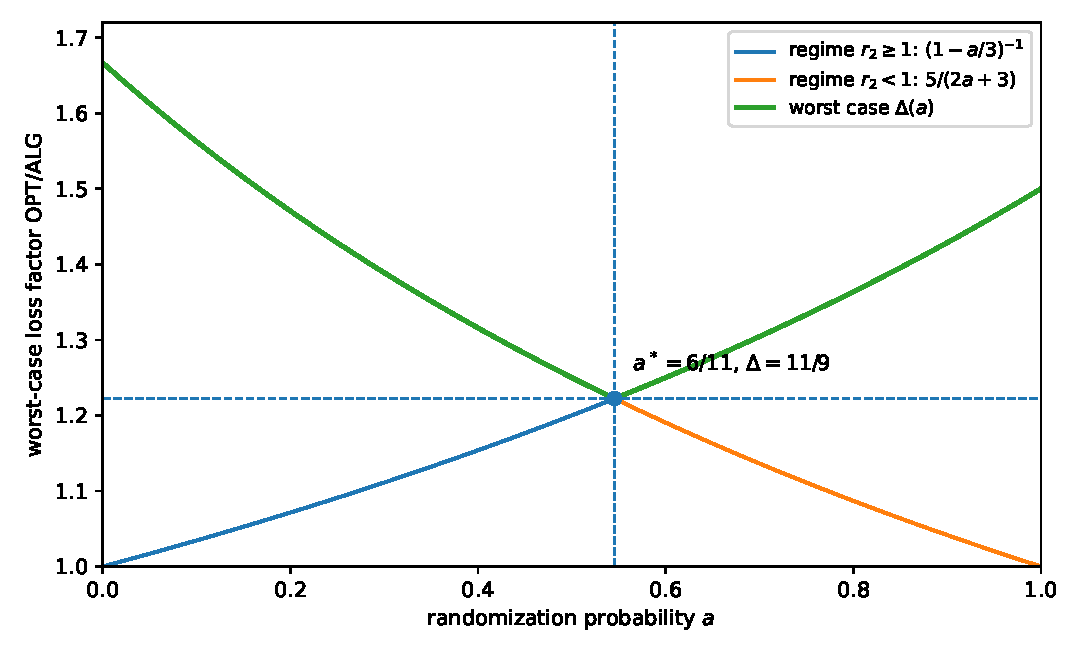
\includegraphics[width=0.85\textwidth]{minimax_n2.pdf}
\caption{The two-period robust example of Proposition~\ref{prop:n2-randomized}.
The randomized rule balances the two adversarial regimes at \(a^\star=6/11\),
where the worst-case ratio is \(9/11\).}
\end{figure}

\subsection{Exact randomized minimax formulation}

For general \(n\), one should not expect a closed-form minimax randomized rule
of the same simplicity as Bruss' threshold.  Nevertheless, the exact robust
randomized problem has a clean finite-dimensional/semi-infinite formulation.
Let
\[
  \mathcal U
  =
  \prod_{i=1}^n
  \left[\frac{\bar r_i}{\rho},\rho\bar r_i\right]
\]
be the uncertainty set for the true odds.  For a true instance
\(r=(r_1,\dots,r_n)\), define the value of the deterministic threshold \(s\) by
\[
  V_s(r)
  =
  \left(\prod_{j=s}^n\frac1{1+r_j}\right)
  \left(\sum_{j=s}^n r_j\right).
\]
By Bruss' theorem,
\[
  V^\star(r)=\max_{1\le s\le n}V_s(r).
\]

Let \(\mathcal D_n\) be the finite set of deterministic stopping rules on the
binary tree of histories.  For \(d\in\mathcal D_n\), let \(W_d(r)\) be the
probability that rule \(d\) stops on the last success under true odds \(r\).  A
mixed randomized rule is a distribution \(z\in\Delta(\mathcal D_n)\).  Its value
on instance \(r\) is
\[
  W_z(r)=\sum_{d\in\mathcal D_n}z_d W_d(r).
\]
Thus the exact randomized minimax ratio is
\[
  \Gamma_n^\star
  =
  \max_{z\in\Delta(\mathcal D_n)}
  \inf_{r\in\mathcal U}
  \frac{W_z(r)}{V^\star(r)}.
\]
Equivalently, \(\Gamma_n^\star\) is the value of the semi-infinite linear program
\[
\begin{aligned}
  \text{maximize}\quad & \gamma \\
  \text{over}\quad & z\in\Delta(\mathcal D_n),\quad \gamma\ge0 \\
  \text{subject to}\quad
  & \sum_{d\in\mathcal D_n}z_d W_d(r)
    \ge \gamma V_s(r),
    \\
  & \hspace{5em}\forall r\in\mathcal U,
    \quad \forall s\in\{1,\dots,n\}.
\end{aligned}
\]
Indeed, the constraints for all \(s\) are equivalent to
\[
  W_z(r)
  \ge
  \gamma\max_s V_s(r)
  =
  \gamma V^\star(r)
  \qquad
  \forall r\in\mathcal U.
\]

This formulation is exact but usually not closed-form.  A practical approach is
a cutting-plane algorithm: start with finitely many scenarios \(r\), solve the
resulting finite linear program, then search for a new scenario and threshold
\(s\) violating the constraint most strongly.  Adding this scenario and
iterating gives increasingly tight randomized minimax rules.  The two-period
calculation above is the smallest case where this program can be solved by hand.

\subsection{Naive target versus robust target}

The naive idea is to ignore robustness and still target a predicted tail-odds
sum of one:
\[
  \theta=1.
\]
Then \(x=\rho\), and the robust discrete theorem gives
\[
  \frac{W_{\mathrm{naive}}}{V^\star}
  \ge
  \min\left\{\frac1\rho,
  \left(1+\frac{\rho-1}{n-1}\right)^{-(n-1)}\right\}.
\]
For \(\rho\ge1\),
\[
  \left(1+\frac{\rho-1}{n-1}\right)^{n-1}\ge 1+(\rho-1)=\rho,
\]
so the second term is the smaller one.  Therefore the finite-\(n\) naive
guarantee is
\[
  \boxed{
  \beta_n(\rho)
  =
  \left(1+\frac{\rho-1}{n-1}\right)^{-(n-1)}.
  }
  \tag{5}
\]

By contrast, the optimized robust target uses
\[
  \theta_n^\star(\rho)=\frac{x_n^\star(\rho)}{\rho}.
\]
For \(\rho>1\), one has \(1<x_n^\star(\rho)<\rho\), hence
\[
  \theta_n^\star(\rho)<1.
\]
Thus robustification starts slightly later than the naive predicted-Bruss rule.
The reason is intuitive: if the true odds are larger than predicted, then
starting at predicted mass one is too early and risks stopping on a success that
is not the last.

\subsection{Large-\(n\) limit}

Let \(n\to\infty\).  For fixed \(x\),
\[
  \left(1+\frac{x-1}{n-1}\right)^{n-1}\to \e^{x-1}.
\]
Hence \((2)\) converges to
\[
  x\e^{x-1}=\rho^2.
\]
Equivalently,
\[
  x\e^x=\e\rho^2.
\]
Therefore
\[
  \boxed{
  x_\infty^\star(\rho)=\LambertW(\e\rho^2),
  \qquad
  \theta_\infty^\star(\rho)=\frac{\LambertW(\e\rho^2)}{\rho},
  \qquad
  \alpha_\infty(\rho)=\frac{\LambertW(\e\rho^2)}{\rho^2}.
  }
  \tag{6}
\]
The naive asymptotic guarantee is
\[
  \boxed{
  \beta_\infty(\rho)=\e^{1-\rho}.
  }
  \tag{7}
\]
For large \(\rho\),
\[
  \alpha_\infty(\rho)
  =\frac{\LambertW(\e\rho^2)}{\rho^2}
  \sim
  \frac{2\log\rho}{\rho^2},
\]
whereas
\[
  \beta_\infty(\rho)=\e^{1-\rho}
\]
decays exponentially in \(\rho\).  Thus the robust target can be substantially
better than blindly targeting one predicted odds unit.

\begin{table}[ht]
\centering
\caption{Discrete independent model.  Optimized robust target versus naive target.}
\begin{tabular}{c c c c c c c}
\toprule
\(\rho\)
& \(\theta^\star_{10}\)
& \(\alpha_{10}\)
& \(\beta_{10}\)
& \(\theta^\star_\infty\)
& \(\alpha_\infty\)
& \(\beta_\infty\)\\
\midrule
1 & 1.000 & 1.000 & 1.000 & 1.000 & 1.000 & 1.000 \\
1.25 & 0.989 & 0.792 & 0.781 & 0.988 & 0.790 & 0.779 \\
1.5 & 0.967 & 0.645 & 0.615 & 0.962 & 0.642 & 0.607 \\
2 & 0.911 & 0.455 & 0.387 & 0.900 & 0.450 & 0.368 \\
3 & 0.805 & 0.268 & 0.164 & 0.782 & 0.261 & 0.135 \\
5 & 0.656 & 0.131 & 0.037 & 0.618 & 0.124 & 0.018 \\
10 & 0.465 & 0.047 & 0.002 & 0.418 & 0.042 & 0.000 \\
\bottomrule
\end{tabular}
\end{table}

\begin{figure}[ht]
\centering
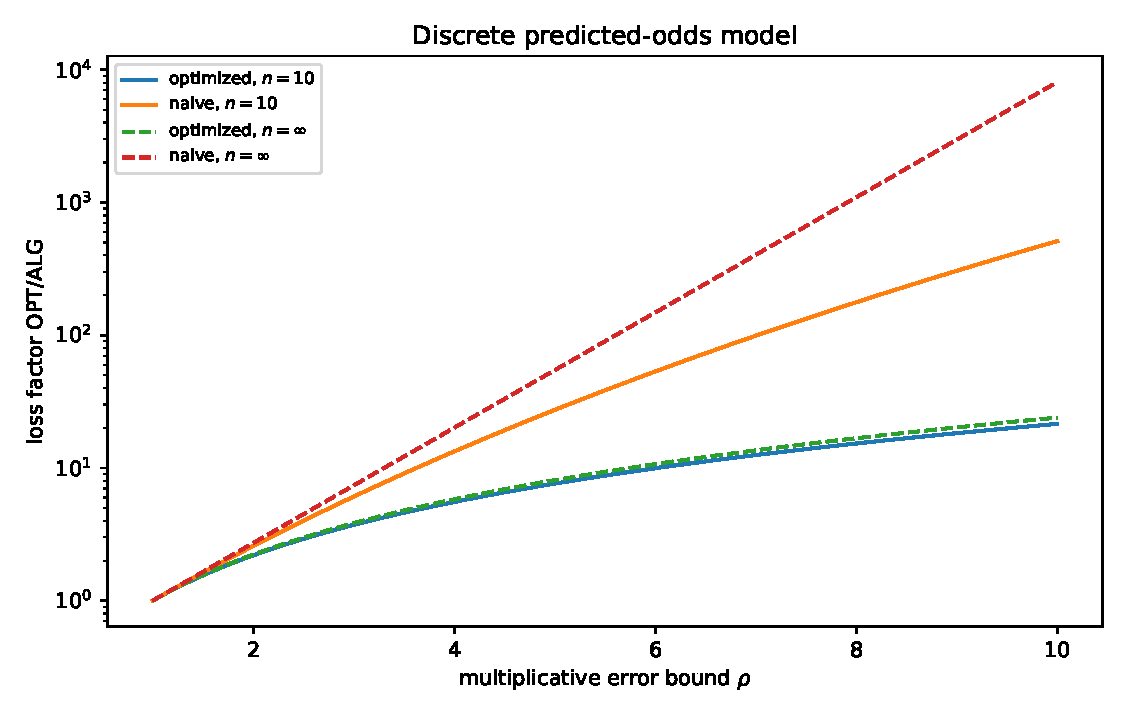
\includegraphics[width=0.95\textwidth]{discrete_ratios.pdf}
\caption{Discrete independent case: optimized robust target versus the naive target.}
\end{figure}

\section{Continuous Poisson model}

We now move to the continuous model discussed by Bruss.  Let successes arrive on
\([0,T]\) according to an inhomogeneous Poisson process with true intensity
\(\varphi(t)\).  Define the true remaining mass
\[
  M(t)=\int_t^T\varphi(u)\,du.
\]
If we start accepting at time \(t\) and then stop at the first success after
\(t\), we win if and only if there is exactly one success after \(t\).  Since the
number of future successes is Poisson with mean \(M(t)\),
\[
  W(t)=\mathbb P(\Pois(M(t))=1)=M(t)\e^{-M(t)}.
\]
The function \(m\mapsto m\e^{-m}\) is maximized at \(m=1\), with value \(1/\e\).
Thus, when the intensity is known, the optimal rule is
\[
  \boxed{
  \int_\tau^T\varphi(u)\,du=1,
  \quad\text{then stop at the first success after }\tau.
  }
  \tag{8}
\]

\subsection{Robust intensity prediction}

Suppose now that only a predicted intensity \(\bar\varphi(t)\) is known, and that
\[
  \boxed{
  \frac1\rho\bar\varphi(t)\le\varphi(t)\le\rho\bar\varphi(t)
  }
  \qquad\text{for every }t\in[0,T].
  \tag{B}
\]
Let
\[
  \bar M(t)=\int_t^T\bar\varphi(u)\,du.
\]
A target \(\theta\) means choosing \(\tau_\theta\) such that
\[
  \bar M(\tau_\theta)=\theta,
\]
and then stopping at the first success after \(\tau_\theta\).  By \((B)\), the
true remaining mass satisfies
\[
  M(\tau_\theta)\in\left[\frac{\theta}{\rho},\rho\theta\right].
\]
Since the omniscient optimum has value \(1/\e\), the guaranteed ratio of target
\(\theta\) is
\[
  e\min_{m\in[\theta/\rho,\rho\theta]}m\e^{-m}.
\]

\begin{theorem}[Optimal robust Poisson target]
\label{thm:poisson-robust}
For \(\rho>1\), the robustly optimal target is
\[
  \boxed{
  \theta^\star_{\mathrm P}(\rho)
  =
  \frac{2\rho\log\rho}{\rho^2-1}.
  }
  \tag{9}
\]
The continuous extension gives \(\theta^\star_{\mathrm P}(1)=1\).  The resulting
worst-case ratio against the omniscient optimum \(1/\e\) is
\[
  \boxed{
  \alpha_{\mathrm P}(\rho)
  =
  \frac{2\log\rho}{\rho^2-1}
  \exp\left(1-\frac{2\log\rho}{\rho^2-1}\right).
  }
  \tag{10}
\]
\end{theorem}

\begin{proof}
Let
\[
  f(m)=m\e^{-m}.
\]
Then \(f\) is strictly increasing on \((0,1)\), strictly decreasing on
\((1,\infty)\), and maximized at \(m=1\).

Set
\[
  a=\frac{\theta}{\rho},
  \qquad
  b=\rho\theta=\rho^2a.
\]
For a fixed \(a\), the uncertainty interval for the true mass is \([a,b]\).  The
robust value before multiplying by \(\e\) is
\[
  \min_{m\in[a,b]}f(m).
\]
We consider three possible regimes.

\medskip
\noindent\emph{Regime 1: \(b\le1\).}
Then the whole interval lies to the left of the maximizer.  Since \(f\) is
increasing on \((0,1)\), the minimum is \(f(a)\).  Increasing \(a\) increases
\(f(a)\) while preserving \(b\le1\) until \(b=1\).  Thus the best point in this
regime is \(b=1\), i.e. \(a=1/\rho^2\).

\medskip
\noindent\emph{Regime 2: \(a\ge1\).}
Then the whole interval lies to the right of the maximizer.  Since \(f\) is
decreasing on \((1,\infty)\), the minimum is \(f(b)\).  Decreasing \(a\) decreases
\(b=\rho^2a\), hence increases \(f(b)\), until \(a=1\).  Thus the best point in
this regime is \(a=1\).

\medskip
\noindent\emph{Regime 3: \(a<1<b\).}
Then the minimum is
\[
  \min\{f(a),f(b)\}.
\]
As \(a\) increases inside this regime, \(f(a)\) increases and
\(f(b)=f(\rho^2a)\) decreases.  Hence the max-min point is where the two endpoint
values are equal:
\[
  f(a)=f(\rho^2a).
\]
This is
\[
  a\e^{-a}=\rho^2a\e^{-\rho^2a}.
\]
Since \(a>0\), cancellation gives
\[
  1=\rho^2\e^{-(\rho^2-1)a}.
\]
Taking logarithms yields
\[
  a^\star=\frac{2\log\rho}{\rho^2-1}.
\]
Therefore
\[
  \theta^\star_{\mathrm P}=\rho a^\star
  =\frac{2\rho\log\rho}{\rho^2-1}.
\]

It remains only to check that this point indeed lies in Regime 3.  We need
\[
  \frac1{\rho^2}<a^\star<1.
\]
The upper bound is equivalent to
\[
  2\log\rho<\rho^2-1,
\]
which holds strictly for \(\rho>1\).  The lower bound is equivalent to
\[
  \rho^2\log(\rho^2)>\rho^2-1,
\]
or, with \(y=\rho^2>1\),
\[
  y\log y>y-1,
\]
which also holds for \(y>1\).  Thus the equalizing point is feasible and it
beats the boundary optima of the other regimes.

Finally, at the optimum the worst endpoint is
\[
  a^\star=\frac{2\log\rho}{\rho^2-1}.
\]
The guaranteed probability is \(a^\star\e^{-a^\star}\), and the ratio against the
omniscient value \(1/\e\) is
\[
  \e a^\star\e^{-a^\star}
  =a^\star\exp(1-a^\star),
\]
which is exactly \((10)\).
\end{proof}

\subsection{Naive Poisson target}

The naive rule targets \(\bar M(t)=1\).  Then the true remaining mass lies in
\[
  \left[\frac1\rho,\rho\right].
\]
The guaranteed ratio is therefore
\[
  \boxed{
  \beta_{\mathrm P}(\rho)
  =
  \min\left\{
    \frac1\rho\exp\left(1-\frac1\rho\right),
    \rho\e^{1-\rho}
  \right\}.
  }
  \tag{11}
\]
The optimized robust target satisfies
\[
  \theta^\star_{\mathrm P}(\rho)<1
  \qquad(\rho>1),
\]
so, as in the discrete case, robustness means starting slightly later than the
naive predicted-Bruss rule.

\begin{table}[ht]
\centering
\caption{Continuous Poisson model.  Optimized robust target versus naive target.}
\begin{tabular}{c c c c}
\toprule
\(\rho\)
& \(\theta^\star_{\mathrm P}\)
& \(\alpha_{\mathrm P}\)
& \(\beta_{\mathrm P}\)\\
\midrule
1 & 1.000 & 1.000 & 1.000 \\
1.25 & 0.992 & 0.975 & 0.974 \\
1.5 & 0.973 & 0.922 & 0.910 \\
2 & 0.924 & 0.791 & 0.736 \\
3 & 0.824 & 0.567 & 0.406 \\
5 & 0.671 & 0.319 & 0.092 \\
10 & 0.465 & 0.121 & 0.001 \\
\bottomrule
\end{tabular}
\end{table}

\begin{figure}[ht]
\centering
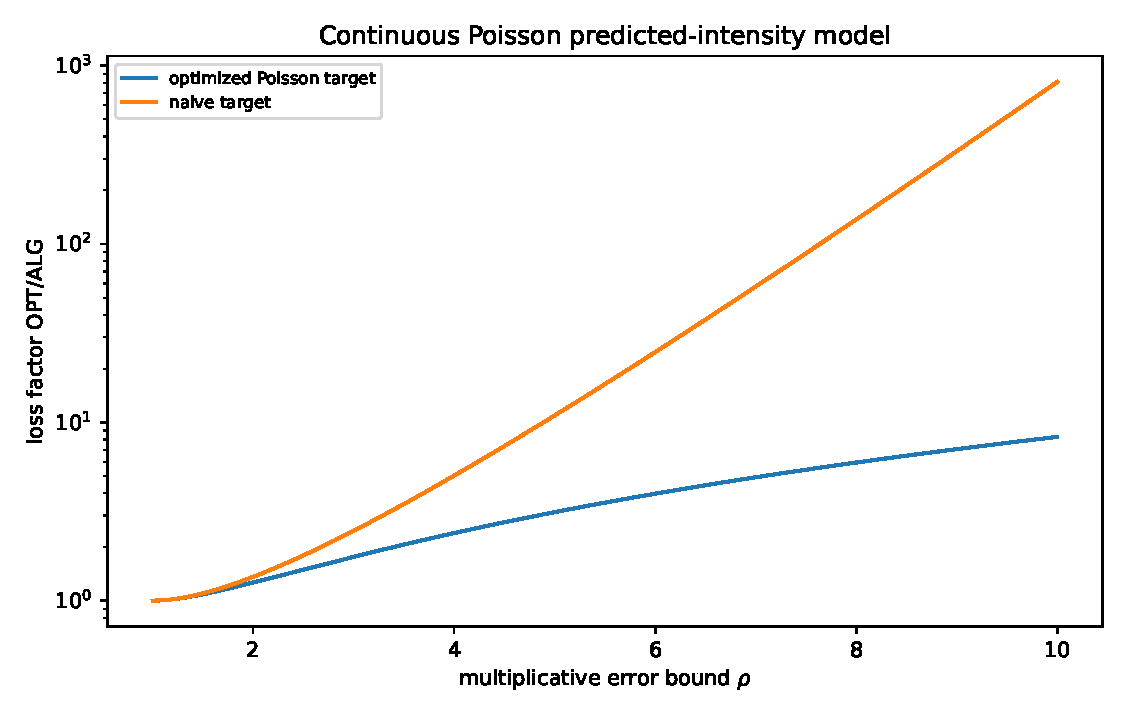
\includegraphics[width=0.95\textwidth]{poisson_ratios.pdf}
\caption{Continuous Poisson case: optimized robust target versus the naive target.}
\end{figure}

\begin{figure}[ht]
\centering
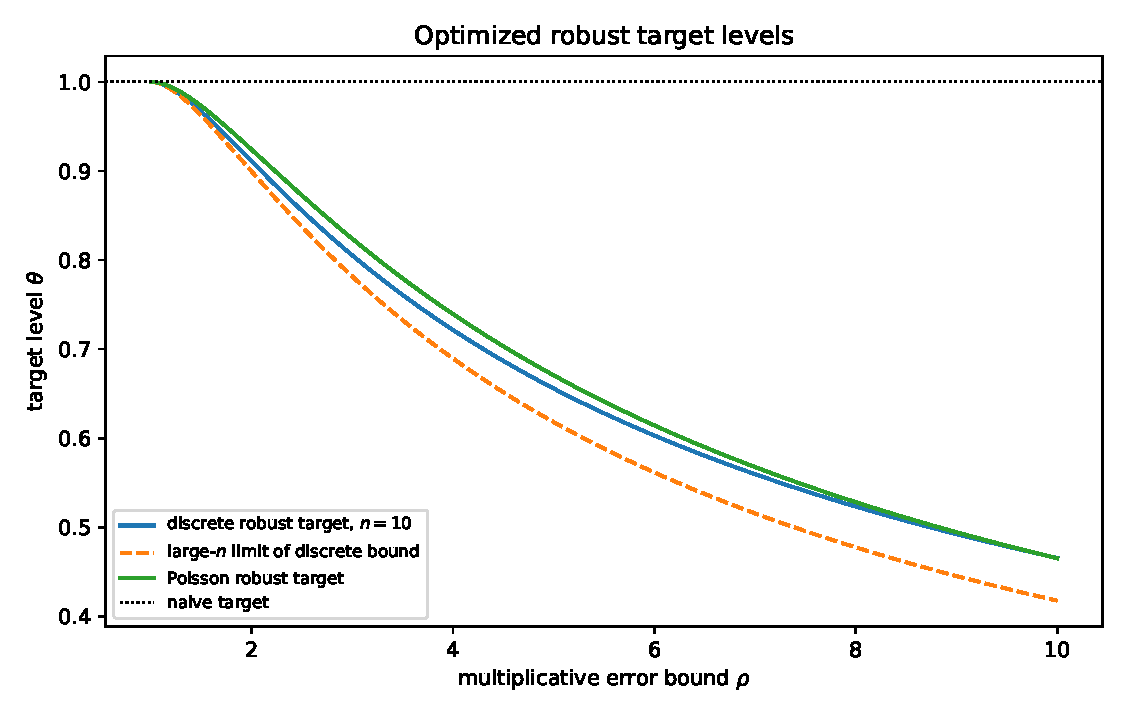
\includegraphics[width=0.95\textwidth]{targets.pdf}
\caption{Optimized target levels.  Both robust targets are below \(1\) as soon as
\(\rho>1\): with uncertainty, one should start slightly later than the naive
predicted-Bruss rule.}
\end{figure}

\section{Bayesian random multiplicative errors on the odds}
\label{sec:bayes-random-errors}

The preceding sections treated a worst-case multiplicative uncertainty set.  We
now consider a different, genuinely Bayesian, model.  The prediction error is no
longer bounded by a known factor and chosen adversarially.  Instead, each local
prediction error is drawn independently from a known law.

\subsection{Model 2: independent random multiplicative errors}

The model is the following.  We observe predicted odds
\[
  \bar r_1,\dots,\bar r_n>0.
\]
For each time $i$, a hidden multiplicative error $\rho_i$ is drawn independently
from a known probability law $\mathcal R$ on $(0,\infty)$, and the true odd is
\[
  \boxed{
  r_i=\frac{\bar r_i}{\rho_i}.
  }
  \tag{12}
\]
Equivalently, the prediction is
\[
  \bar r_i=r_i\rho_i.
\]
Conditionally on $\rho_i$, the true success probability at time $i$ is therefore
\[
  p_i(\rho_i)
  =\frac{r_i}{1+r_i}
  =\frac{\bar r_i/\rho_i}{1+\bar r_i/\rho_i}
  =\frac{\bar r_i}{\rho_i+\bar r_i}.
\]
The indicators $I_1,\dots,I_n$ are generated independently conditionally on the
hidden errors $\rho_1,
\dots,\rho_n$.

The objective is the Bayesian one: maximize the conditional, ex ante probability
of stopping on the last success given the observed predictions
$\bar r_1,
\dots,\bar r_n$ and the known error law $\mathcal R$.

\begin{remark}[Local errors versus a global error]
This section uses independent local errors $\rho_i$.  This assumption is crucial.
If instead a single unknown factor $\rho$ were shared by all times, then the
observed successes and failures would update the posterior distribution of
$\rho$, and the problem would become a dynamic program on that posterior.  The
simple reduction below would no longer apply.
\end{remark}

\subsection{The induced Bernoulli probabilities}

Define the Bayesian marginal probability of success at time $i$ by
\[
  \pi_i
  =\mathbb E_{\rho\sim\mathcal R}
  \left[
    \frac{\bar r_i}{\rho+\bar r_i}
  \right].
\]
Then
\[
  1-\pi_i
  =\mathbb E_{\rho\sim\mathcal R}
  \left[
    \frac{\rho}{\rho+\bar r_i}
  \right].
\]
The corresponding Bayesian effective odd is
\[
  \boxed{
  b_i
  :=\frac{\pi_i}{1-\pi_i}
  =
  \frac{
    \mathbb E_{\rho\sim\mathcal R}
    \left[\dfrac{\bar r_i}{\rho+\bar r_i}\right]
  }{
    \mathbb E_{\rho\sim\mathcal R}
    \left[\dfrac{\rho}{\rho+\bar r_i}\right]
  }.
  }
  \tag{13}
\]

\begin{lemma}[Marginal independence after integrating the local errors]
\label{lem:marginal-independence}
Under Model 2, conditional on the predictions $\bar r_1,
\dots,\bar r_n$, the
indicators $I_1,\dots,I_n$ are independent Bernoulli random variables with
success probabilities $\pi_1,
\dots,\pi_n$.
\end{lemma}

\begin{proof}
Fix a vector $\varepsilon=(\varepsilon_1,
\dots,\varepsilon_n)\in\{0,1\}^n$.
Conditionally on the hidden errors, the indicators are independent, hence
\[
  \mathbb P(I_1=\varepsilon_1,
\dots,I_n=\varepsilon_n\mid \rho_1,
\dots,\rho_n)
  =
  \prod_{i=1}^n
  p_i(\rho_i)^{\varepsilon_i}
  \bigl(1-p_i(\rho_i)\bigr)^{1-\varepsilon_i}.
\]
Taking expectation over the independent hidden errors $\rho_i$ factorizes the
right-hand side:
\begin{align*}
  \mathbb P(I_1=\varepsilon_1,
\dots,I_n=\varepsilon_n)
  &=
  \prod_{i=1}^n
  \mathbb E\left[
    p_i(\rho_i)^{\varepsilon_i}
    \bigl(1-p_i(\rho_i)\bigr)^{1-\varepsilon_i}
  \right] \\
  &=
  \prod_{i=1}^n
  \pi_i^{\varepsilon_i}(1-\pi_i)^{1-\varepsilon_i}.
\end{align*}
This is exactly the joint law of independent Bernoulli variables with parameters
$\pi_i$.
\end{proof}

\begin{theorem}[Bayesian odds theorem under independent local errors]
\label{thm:bayes-bruss}
Under Model 2, the Bayesian optimal rule is obtained by applying Bruss' odds
algorithm to the effective odds $b_i$ defined in \((13)\).  That is, define
\[
  B_k=\sum_{j=k}^n b_j,
  \qquad
  \widetilde Q_k=\prod_{j=k}^n(1-\pi_j),
\]
with $B_{n+1}=0$.  In the non-degenerate case $B_1>1$, let
\[
  s_{\mathcal R}
  =\sup\left\{k:B_k\ge1\right\}.
\]
Then the Bayesian optimal rule ignores successes before $s_{\mathcal R}$ and
stops at the first success from $s_{\mathcal R}$ onward.  Its Bayesian value is
\[
  \boxed{
  V_{\mathcal R}^{\star}
  =\widetilde Q_{s_{\mathcal R}}B_{s_{\mathcal R}}.
  }
  \tag{14}
\]
If $B_1<1$, the Bayesian optimal rule stops at the first success from the
beginning.
\end{theorem}

\begin{proof}
By Lemma~\ref{lem:marginal-independence}, after the hidden local errors have
been integrated out, the Bayesian problem conditional on the predictions is an
ordinary independent Bernoulli last-success problem with success probabilities
$\pi_i$.  Its odds are precisely
\[
  \frac{\pi_i}{1-\pi_i}=b_i.
\]
Bruss' odds theorem therefore applies verbatim to the sequence
$\pi_1,
\dots,\pi_n$.  It says to sum the odds $b_i$ from the end until reaching one,
and then stop at the first success from that index onward.  The value formula is
the usual threshold value formula
\[
  \left(\prod_{j=s_{\mathcal R}}^n(1-\pi_j)\right)
  \left(\sum_{j=s_{\mathcal R}}^n b_j\right)
  =\widetilde Q_{s_{\mathcal R}}B_{s_{\mathcal R}}.
\]
This proves the claim.
\end{proof}

\subsection{The calibration map}

It is useful to view the theorem as a deterministic calibration of the predicted
odds.  For $x>0$, define
\[
  M_{\mathcal R}(x)
  =\mathbb E_{\rho\sim\mathcal R}\left[\frac1{\rho+x}\right].
\]
Then
\[
  \pi(x)=xM_{\mathcal R}(x),
  \qquad
  1-\pi(x)=1-xM_{\mathcal R}(x),
\]
and the effective odd associated with a predicted odd $x$ is
\[
  \boxed{
  B_{\mathcal R}(x)
  =\frac{xM_{\mathcal R}(x)}{1-xM_{\mathcal R}(x)}.
  }
  \tag{15}
\]
Thus Model 2 is algorithmically simple:
\[
  \boxed{
  \bar r_i\quad\longmapsto\quad B_{\mathcal R}(\bar r_i),
  \quad\text{then apply Bruss to these calibrated odds.}
  }
\]

\begin{lemma}[Basic properties of the calibration map]
\label{lem:calibration-properties}
For any law $\mathcal R$ on $(0,\infty)$, the map
$x\mapsto B_{\mathcal R}(x)$ is nondecreasing and finite for every $x>0$.
Moreover, if $\mathbb E[1/\rho]<\infty$, then
\[
  B_{\mathcal R}(x)
  \sim x\mathbb E\left[\frac1\rho\right]
  \qquad (x\downarrow0),
\]
and if $\mathbb E[\rho]<\infty$, then
\[
  B_{\mathcal R}(x)
  \sim \frac{x}{\mathbb E[\rho]}
  \qquad (x\to\infty).
\]
\end{lemma}

\begin{proof}
The function $x\mapsto x/(\rho+x)$ is increasing for every fixed $\rho>0$.
Therefore
\[
  \pi(x)=\mathbb E\left[\frac{x}{\rho+x}\right]
\]
is nondecreasing.  Since $0<x/(\rho+x)<1$ for every $\rho>0$, one has
$0<\pi(x)<1$, hence
\[
  B_{\mathcal R}(x)=\frac{\pi(x)}{1-\pi(x)}
\]
is finite and nondecreasing.

If $\mathbb E[1/\rho]<\infty$, then
\[
  \frac1x\pi(x)
  =\mathbb E\left[\frac1{\rho+x}\right]
  \longrightarrow
  \mathbb E\left[\frac1\rho\right]
\]
by monotone convergence.  Since $\pi(x)\to0$ as $x\downarrow0$, this gives
$B_{\mathcal R}(x)\sim \pi(x)\sim x\mathbb E[1/\rho]$.

If $\mathbb E[\rho]<\infty$, write
\[
  1-\pi(x)=\mathbb E\left[\frac{\rho}{\rho+x}\right].
\]
Then
\[
  x(1-\pi(x))
  =\mathbb E\left[\frac{x\rho}{\rho+x}\right]
  \longrightarrow
  \mathbb E[\rho]
\]
by monotone convergence, because $x\rho/(x+\rho)\uparrow\rho$.  Since
$\pi(x)\to1$, we obtain
\[
  B_{\mathcal R}(x)
  =\frac{\pi(x)}{1-\pi(x)}
  \sim \frac1{1-\pi(x)}
  \sim \frac{x}{\mathbb E[\rho]}.
\]
\end{proof}

\subsection{Examples of error laws}

The only quantity needed by the algorithm is $M_{\mathcal R}(x)$.  For several
simple laws it is explicit.

\paragraph{Deterministic multiplicative error.}
If $\rho\equiv c$, then
\[
  M_{\mathcal R}(x)=\frac1{c+x},
  \qquad
  B_{\mathcal R}(x)=\frac{x}{c}.
\]
This recovers the obvious rescaling of all predicted odds.

\paragraph{Finite mixture.}
If $\rho=c_\ell$ with probability $w_\ell$, where $\sum_\ell w_\ell=1$, then
\[
  M_{\mathcal R}(x)=\sum_\ell\frac{w_\ell}{c_\ell+x},
\]
and therefore
\[
  B_{\mathcal R}(x)
  =
  \frac{
    x\sum_\ell\dfrac{w_\ell}{c_\ell+x}
  }{
    1-x\sum_\ell\dfrac{w_\ell}{c_\ell+x}
  }.
\]
This is often the most practical case numerically: a continuous law can be
approximated by a finite mixture, after which the algorithm is fully explicit.

\paragraph{Uniform law.}
If $\rho\sim\mathrm{Unif}[a,b]$, with $0<a<b$, then
\[
  M_{\mathcal R}(x)
  =\frac1{b-a}\log\left(\frac{b+x}{a+x}\right),
\]
so
\[
  B_{\mathcal R}(x)
  =
  \frac{
    \dfrac{x}{b-a}\log\left(\dfrac{b+x}{a+x}\right)
  }{
    1-\dfrac{x}{b-a}\log\left(\dfrac{b+x}{a+x}\right)
  }.
\]

\paragraph{Gamma law.}
Let $\rho\sim\Gamma(a,\beta)$, where $a>0$ is the shape and $\beta>0$ is the rate:
\[
  f(\rho)=\frac{\beta^a}{\Gamma(a)}\rho^{a-1}e^{-\beta\rho},
  \qquad \rho>0.
\]
Then
\[
  \boxed{
  M_{\mathcal R}(x)
  =
  \beta^a x^{a-1}e^{\beta x}\Gamma(1-a,\beta x),
  }
  \tag{16}
\]
where $\Gamma(\cdot,\cdot)$ denotes the upper incomplete gamma function.  Hence
\[
  \boxed{
  B_{\mathcal R}(x)
  =
  \frac{
    \beta^a x^a e^{\beta x}\Gamma(1-a,\beta x)
  }{
    1-\beta^a x^a e^{\beta x}\Gamma(1-a,\beta x)
  }.
  }
  \tag{17}
\]
For the exponential case $a=1$, this becomes
\[
  M_{\mathcal R}(x)=\beta e^{\beta x}E_1(\beta x),
\]
where
\[
  E_1(y)=\int_y^\infty\frac{e^{-t}}{t}\,dt.
\]

\paragraph{Shifted half-normal law.}
If
\[
  \rho=1+|Z|,
  \qquad
  Z\sim\mathcal N(0,\sigma^2),
\]
then $\rho\ge1$, so the predictions always overestimate the true odds.  In this
case
\[
  \boxed{
  M_{\mathcal R}(x)
  =
  \sqrt{\frac\pi2}\frac1\sigma
  \exp\left(\frac{(x+1)^2}{2\sigma^2}\right)
  \operatorname{erfc}\left(\frac{x+1}{\sqrt2\sigma}\right).
  }
  \tag{18}
\]
Again $B_{\mathcal R}(x)=xM_{\mathcal R}(x)/(1-xM_{\mathcal R}(x))$.

\paragraph{Log-normal law.}
A log-normal law is natural for multiplicative errors:
\[
  \rho=e^Z,
  \qquad Z\sim\mathcal N(\mu,\sigma^2).
\]
Then
\[
  M_{\mathcal R}(x)=\mathbb E\left[\frac1{x+e^Z}\right].
\]
There is no particularly simple closed form in elementary special functions, but
it is a one-dimensional integral and can be computed accurately by quadrature,
for instance by Gauss--Hermite quadrature.  Once the values
$B_{\mathcal R}(\bar r_i)$ are computed, the stopping rule is still exactly the
Bayesian Bruss rule of Theorem~\ref{thm:bayes-bruss}.

\begin{table}[ht]
\centering
\caption{Examples of the Bayesian calibration $B_{\mathcal R}(x)$.  The
exponential law has mean $1$ but large variance and mass near $0$, which inflates
small effective odds.  The shifted half-normal law satisfies $\rho\ge1$, hence it
mostly deflates the predicted odds.}
\begin{tabular}{c c c c c}
\toprule
$x=\bar r$ & $\rho\equiv1$ & $\mathrm{Unif}[0.5,1.5]$ & $\mathrm{Exp}(1)$ & $1+|N(0,0.5^2)|$\\
\midrule
0.1 & 0.100 & 0.109 & 0.252 & 0.085\\
0.5 & 0.500 & 0.530 & 0.857 & 0.438\\
1.0 & 1.000 & 1.044 & 1.477 & 0.899\\
2.0 & 2.000 & 2.058 & 2.606 & 1.853\\
5.0 & 5.000 & 5.071 & 5.762 & 4.803\\
\bottomrule
\end{tabular}
\end{table}

\begin{figure}[ht]
\centering
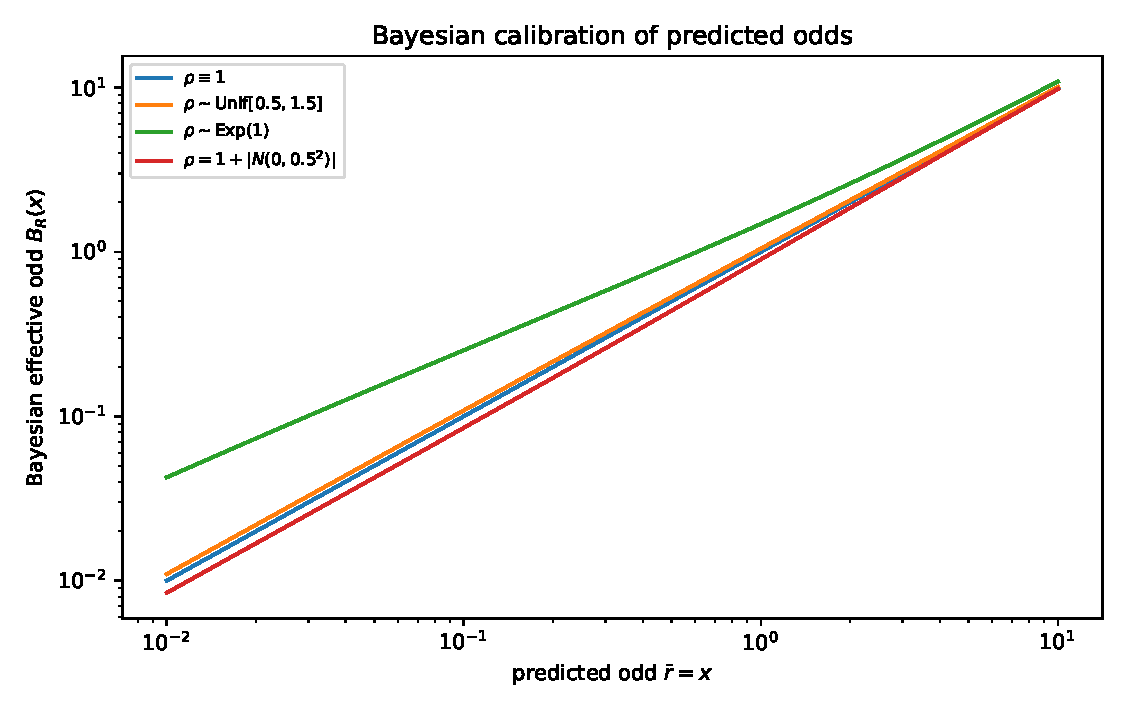
\includegraphics[width=0.95\textwidth]{bayes_calibration.pdf}
\caption{Bayesian calibration map $x\mapsto B_{\mathcal R}(x)$ for several
error laws.  After calibration, the optimal algorithm is simply Bruss' odds rule
applied to the transformed odds.}
\end{figure}

\subsection{What this model buys us}

The worst-case robust model asks for a threshold that performs well for every
realization of the multiplicative error up to a factor $\rho$.  Model 2 asks a
different question: if the local errors are random with known law, what rule
maximizes the Bayesian success probability?  The answer is especially neat:
there is no need for a new stopping theorem.  Random local multiplicative errors
only change the Bernoulli probabilities.  Once those induced probabilities are
computed, Bruss' theorem applies without modification.

In short,
\[
  \boxed{
  \text{random independent local errors }
  \Longrightarrow
  \text{calibrate odds, then sum calibrated odds to one.}
  }
\]


\section{Interpretation}

\paragraph{Known model.}
If the discrete odds \(r_i\) are known, the correct target is
\[
  \sum_{j=s}^n r_j\simeq1.
\]
If the Poisson intensity \(\varphi\) is known, the correct target is
\[
  \int_\tau^T\varphi(u)\,du=1.
\]

\paragraph{Predicted model with multiplicative error.}
If predictions can be wrong by a factor \(\rho\), the naive target \(1\) is too
optimistic.  A robust rule targets a value below \(1\).

In the discrete independent model, the finite-\(n\) robust target is
\[
  \theta_n^\star(\rho)=\frac{x_n^\star(\rho)}{\rho},
  \qquad
  x_n^\star(\rho)
  \left(1+\frac{x_n^\star(\rho)-1}{n-1}\right)^{n-1}=\rho^2.
\]
In the Poisson model, the robust target is
\[
  \theta^\star_{\mathrm P}(\rho)
  =
  \frac{2\rho\log\rho}{\rho^2-1}.
\]

\paragraph{Why the Poisson guarantee is cleaner.}
The Poisson future is summarized by the scalar mass \(M(t)\), and the success
probability is exactly \(M\e^{-M}\).  In the finite discrete case, an atom with a
large odd can create overshoot effects, so the robust finite-\(n\) bound must
also protect against the distribution of mass among finitely many indices.  When
all individual odds are small, the discrete model approaches the smoother
Poisson behavior.

\appendix

\section{Auxiliary inequalities used in the proofs}

\begin{lemma}[Product dominates one plus the sum]
For nonnegative \(u_1,\dots,u_m\),
\[
  \prod_{i=1}^m(1+u_i)\ge1+\sum_{i=1}^m u_i.
\]
\end{lemma}

\begin{proof}
Expand the product.  All terms are nonnegative, and the expansion contains the
constant term \(1\) and the linear terms \(u_1+\cdots+u_m\).
\end{proof}

\begin{lemma}[AM--GM product bound]
If \(z_1,
\dots,z_m\ge0\) and \(z_1+\cdots+z_m\le S\), then
\[
  \prod_{i=1}^m z_i\le\left(\frac{S}{m}\right)^m.
\]
\end{lemma}

\begin{proof}
This is the arithmetic--geometric mean inequality:
\[
  \left(\prod_{i=1}^m z_i\right)^{1/m}
  \le
  \frac1m\sum_{i=1}^m z_i
  \le
  \frac{S}{m}.
\]
Raise both sides to the power \(m\).
\end{proof}

\begin{thebibliography}{9}

\bibitem{Bruss2000}
F. Thomas Bruss.
\newblock Sum the odds to one and stop.
\newblock \emph{The Annals of Probability}, 28(3):1384--1391, 2000.

\end{thebibliography}

\end{document}
